\section{Flujo de trabajo para el versionamiento de programas de estudio}
\begin{table}[H]
\centering
\resizebox{\columnwidth}{!}{%
\begin{tabular}{@{}lllll@{}}
\toprule
Historias de usuario               & HE  & HC  & PH & Sprints \\ \midrule
Información básica del programa    & 54  & 56  & 8  & 1       \\
Competencias de carrera o programa & 48  & 68  & 5  & 1       \\
Bloques de curso                   & 58  & 60  & 5  & 1       \\
Visualizar cambios en los campos   & 180 & 210 & 13 & 4       \\ \bottomrule
\end{tabular}
}
\caption{Historias de usuario para flujo de trabajo para el versionamiento de programas de estudio}
\label{epic:8}
\end{table}

\subsection{Información básica del programa}
La historia de usuario tiene como descripción lo siguiente \enquote{\textit{Como coordinador del departamento o encargado del AMS, me gustaría ser capaz de agregar o revisar programas en el módulo de gestión curricular, para que de esta forma pueda manejar mejor mis registros de la institución en el sistema}}. Y los criterios de aceptación consistían en el desarrollo de la pantalla que se puede apreciar en la figura \ref{program_cover_info}.

Algunas de las tareas identificadas en la planificación de las iteraciones eran los siguientes:
\begin{itemize}
	\item Adaptar la base de datos para soportar los nuevos campos a ser guardados por el flujo de trabajo.
	\item Luego de hacer los cambios en la base de datos, actualizar o agregar nuevas clases de Java para su posterior uso.
	\item Desarrollar la página de información básica del programa.
	\item Actualizar la plantilla de flujos de trabajo institucional para que soporte la creación y revisión de programas.
	\item Diseñar servicios para guardar los registros de la nueva página.
	\item Diseñar servicios de aprobación de flujo de trabajo de programas.
\end{itemize}

La historia fue finalizada en una iteración con una cantidad de 56 horas cargadas en el sistema.

\begin{figure}[H]
\centering
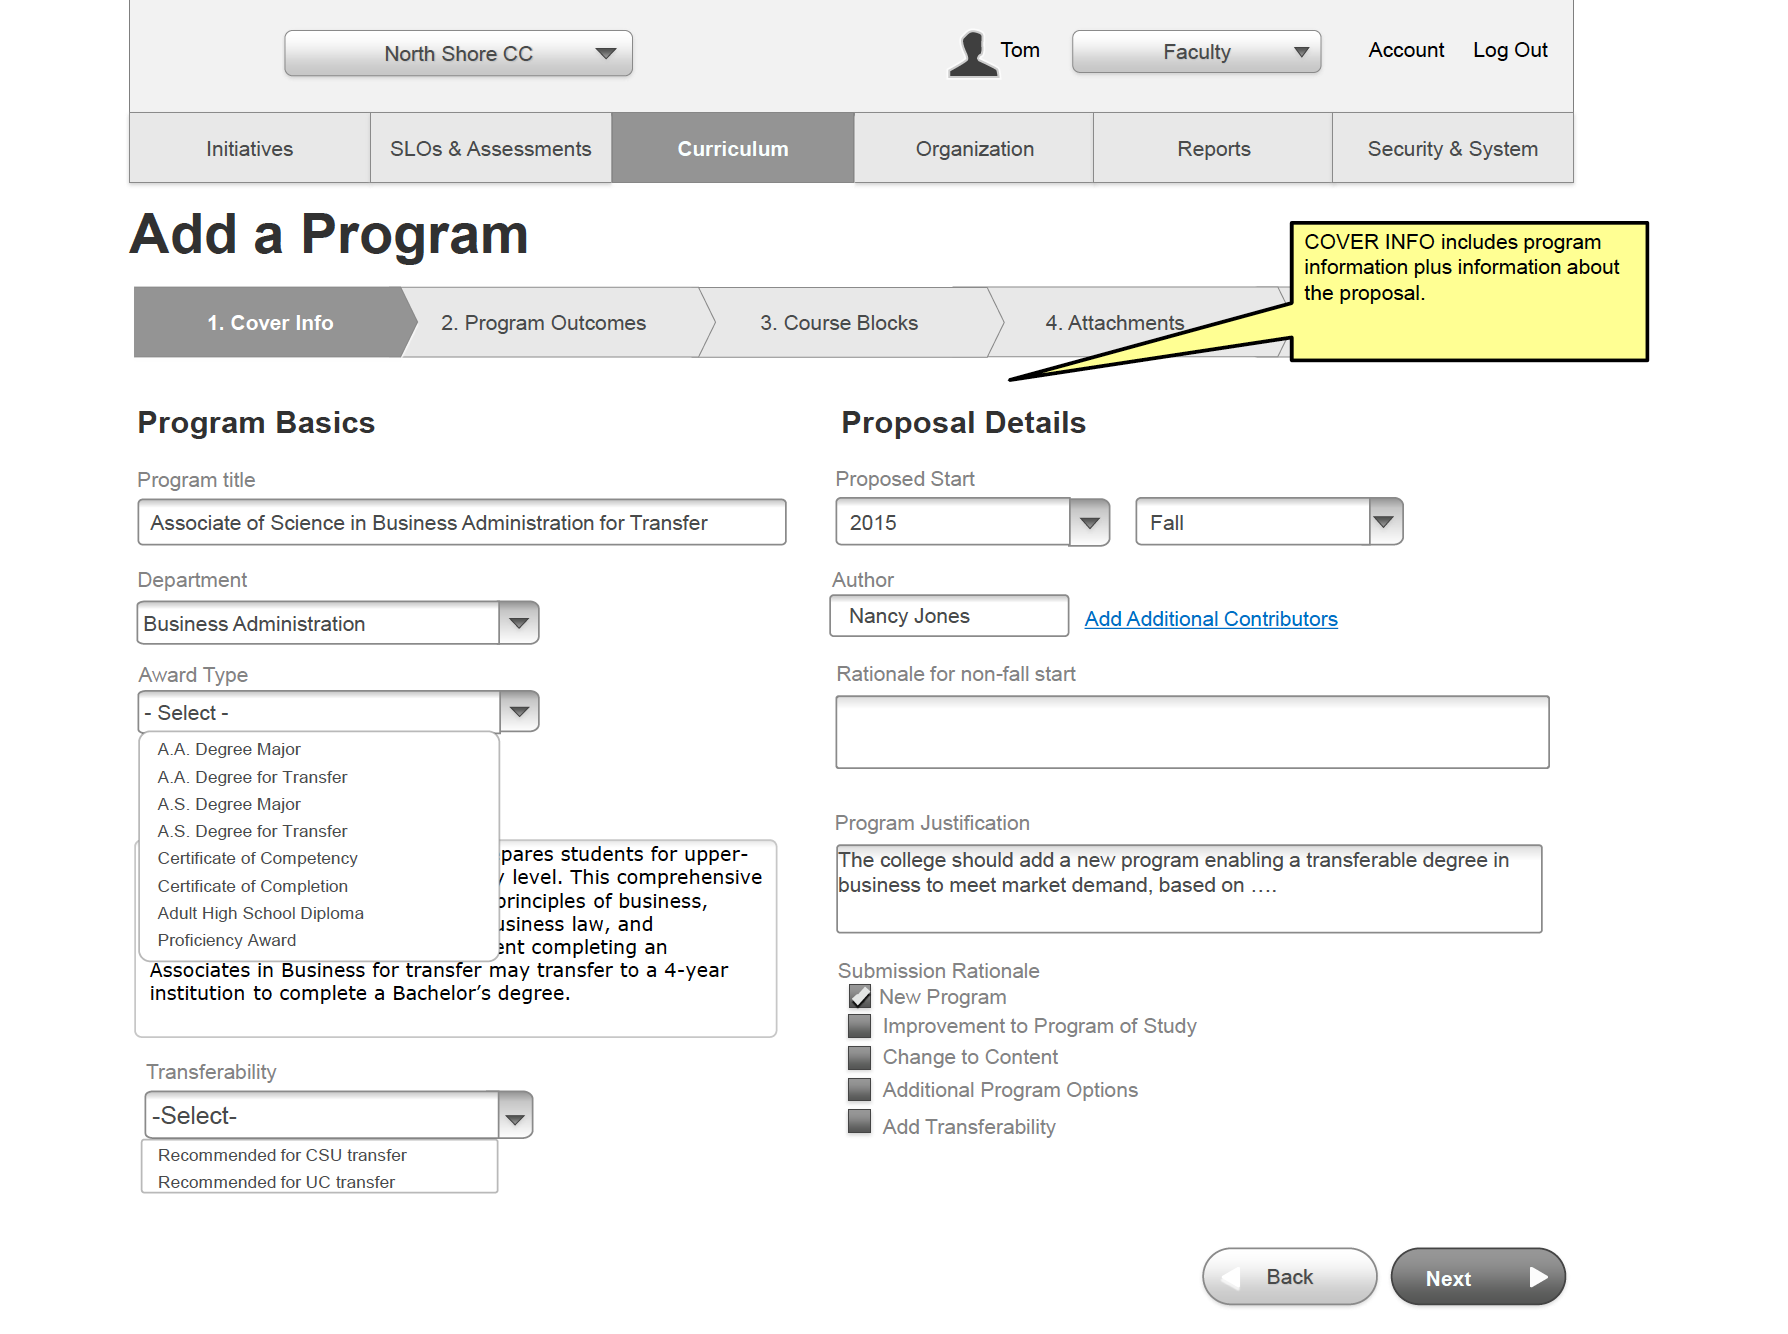
\includegraphics[width=125mm,scale=1]{Capitulos/DesarrollodelaAplicacion/Imagenes/program_cover_info}
\caption{Mockup de la pantalla de información básica del programa.}
  \label{program_cover_info}
\end{figure}

\subsection{Competencias de carrera o programa}
La historia de usuario tiene como descripción lo siguiente \enquote{\textit{Como coordinador, me gustaría ser capaz de administrar las competencias asociadas a mi programas durante el flujo de creación y revisión del mismo, para que pueda hacer una revisión comprensiva de los programas que tiene el AMS}}. Y los criterios de aceptación consistían en el desarrollo de la pantalla que se puede apreciar en la figura \ref{program_learning_outcomes}.

Algunas de las tareas identificadas en la planificación de las iteraciones eran los siguientes:
\begin{itemize}
	\item Adaptar la base de datos para soportar los nuevos campos a ser guardados por el flujo de trabajo.
	\item Luego de hacer los cambios en la base de datos, actualizar o agregar nuevas clases de Java para su posterior uso.
	\item Desarrollar la página de información básica del programa.
	\item Actualizar los servicios de guardado de campos para el flujo de trabajo.
	\item Actualizar los servicios de aprobación de flujo de trabajo de programas.
\end{itemize}

La historia fue finalizada en una iteración con una cantidad de 68 horas cargadas en el sistema.

\begin{figure}[H]
\centering
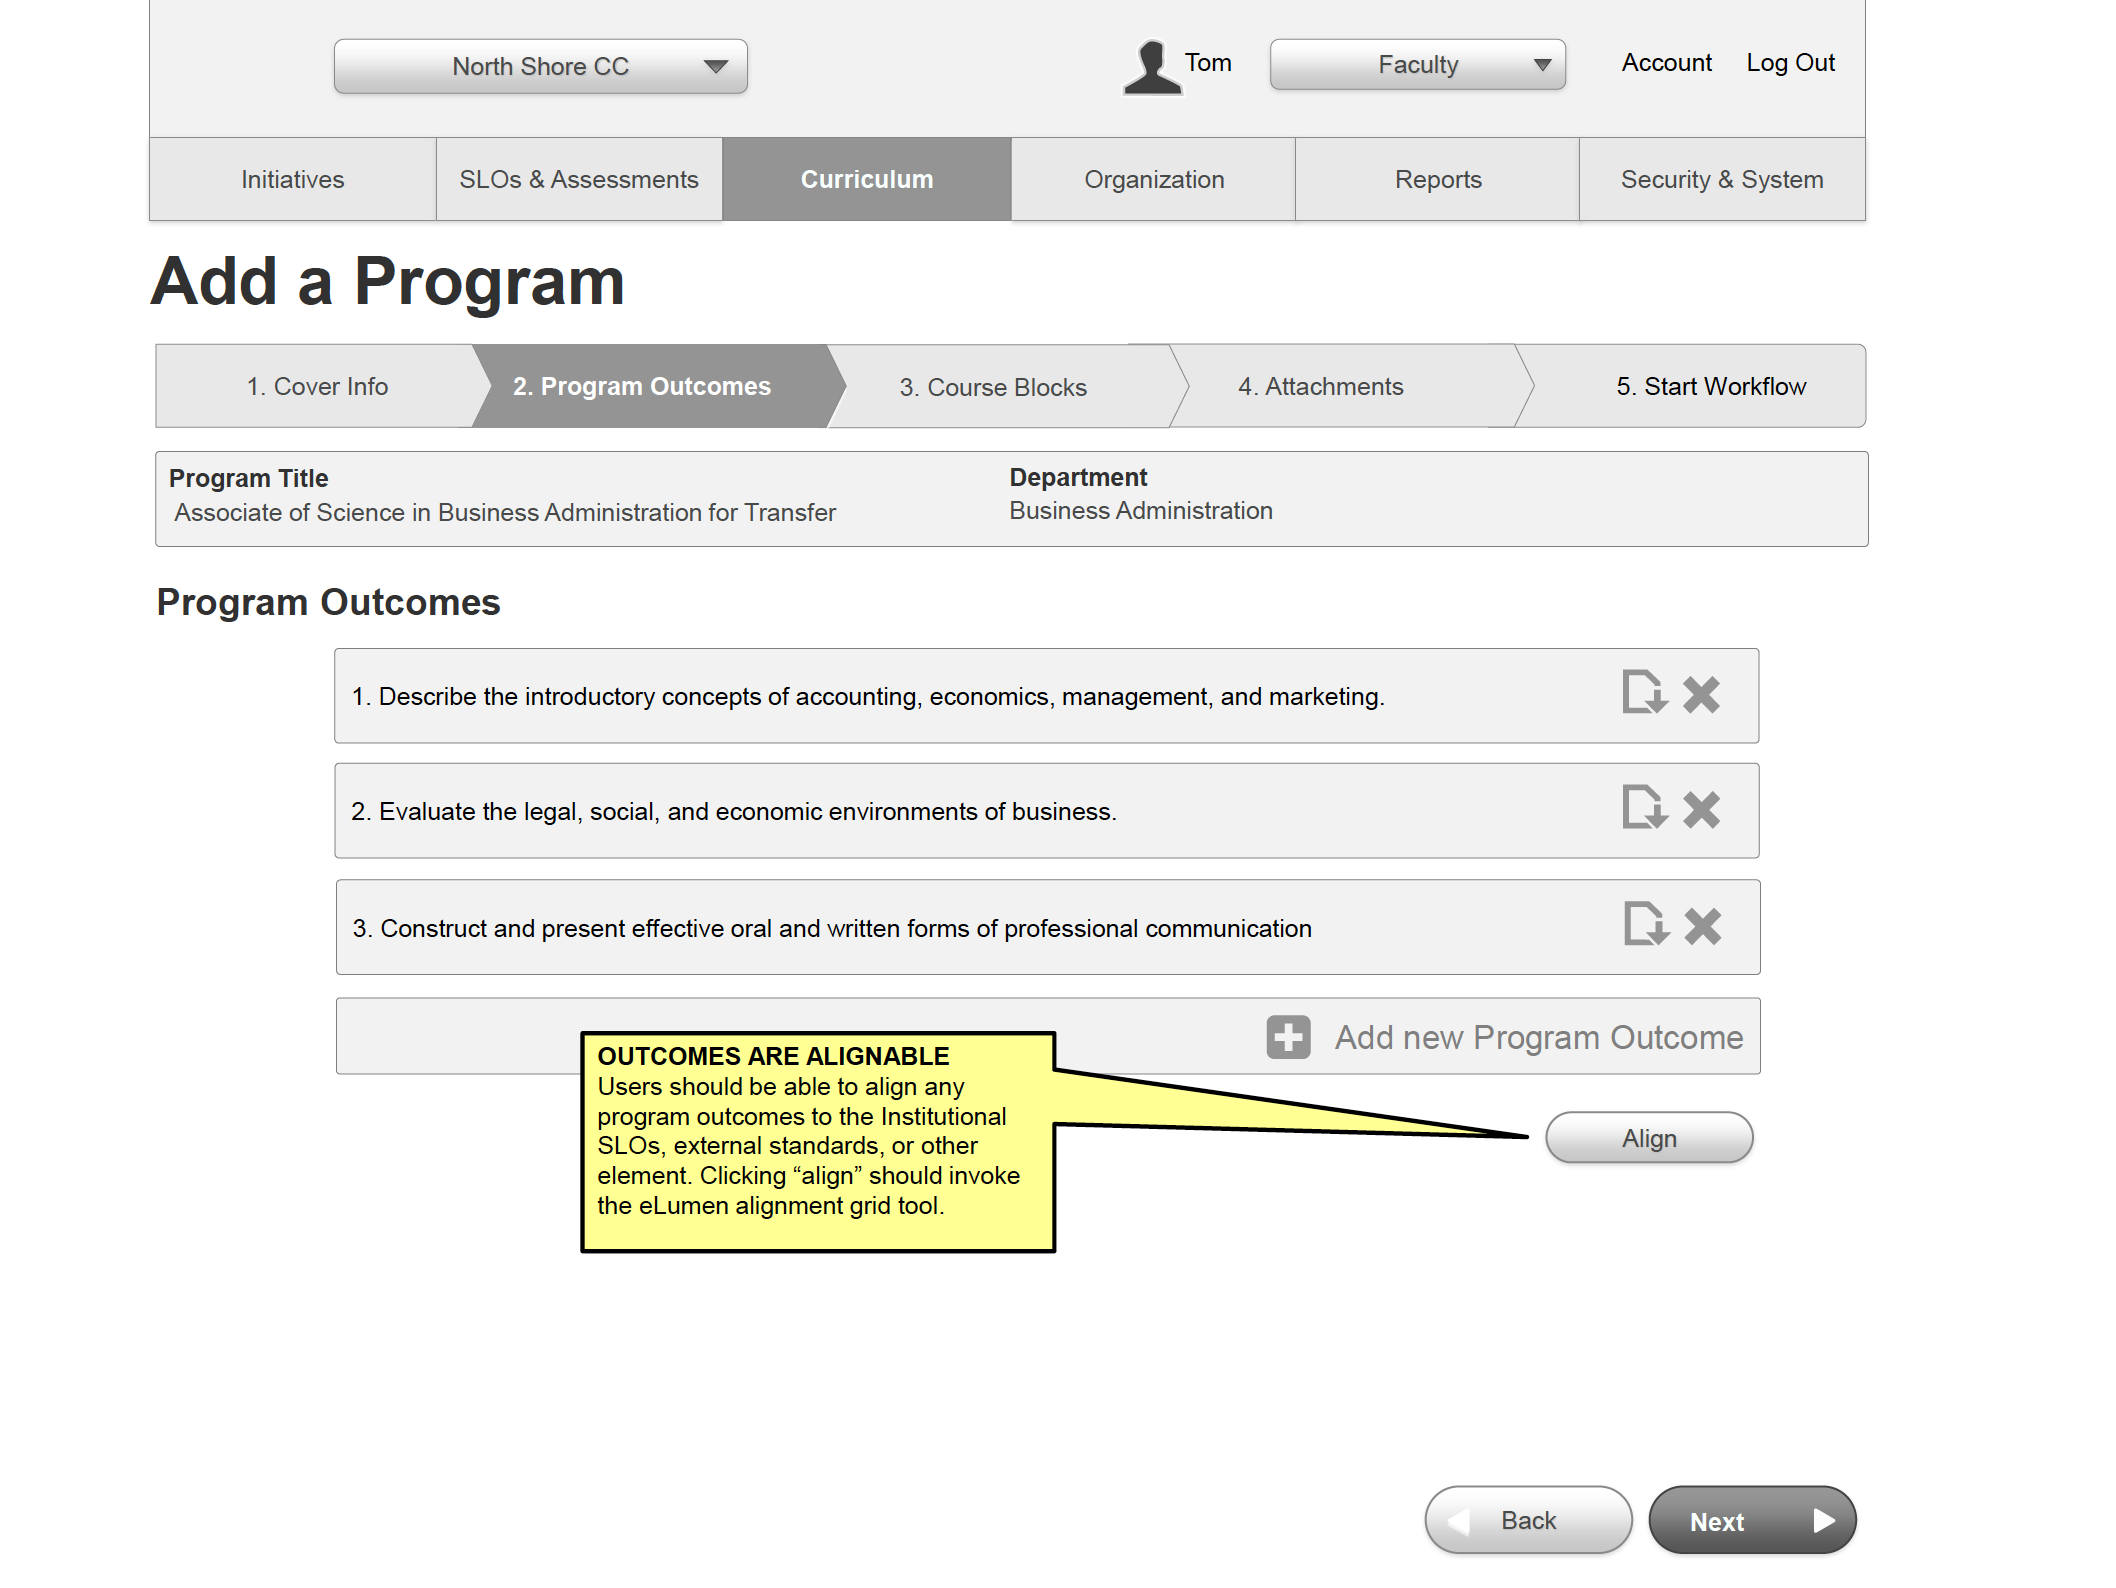
\includegraphics[width=125mm,scale=1]{Capitulos/DesarrollodelaAplicacion/Imagenes/program_learning_outcomes}
\caption{Mockup de la pantalla de competencias del programa.}
  \label{program_learning_outcomes}
\end{figure}

\subsection{Bloques de cursos}
La historia de usuario tiene como descripción lo siguiente \enquote{\textit{Como coordinador de departamento, me gustaría ser capaz de diseñar bloques de cursos para mis programas, para que de esta manera pueda diseñar la malla para mis programas de estudio}}. Y los criterios de aceptación consistían en el desarrollo de la pantalla que se puede apreciar en la figura \ref{program_course_blocks}.

Algunas de las tareas identificadas en la planificación de las iteraciones eran los siguientes:
\begin{itemize}
	\item Diseño e implementación del modelo de datos.
	\item Diseño e implementación de clases Java.
	\item Desarrollar la página de paso para creación de bloques de cursos en los diferentes flujos de trabajo.
	\item Desarrollar servicios de guardado y aprobación de la funcionalidad.
	\item Actualizar la plantilla de flujos de trabajo.
\end{itemize}

La historia fue finalizada en una iteración con una cantidad de 60 horas cargadas en el sistema.

\begin{figure}[H]
\centering
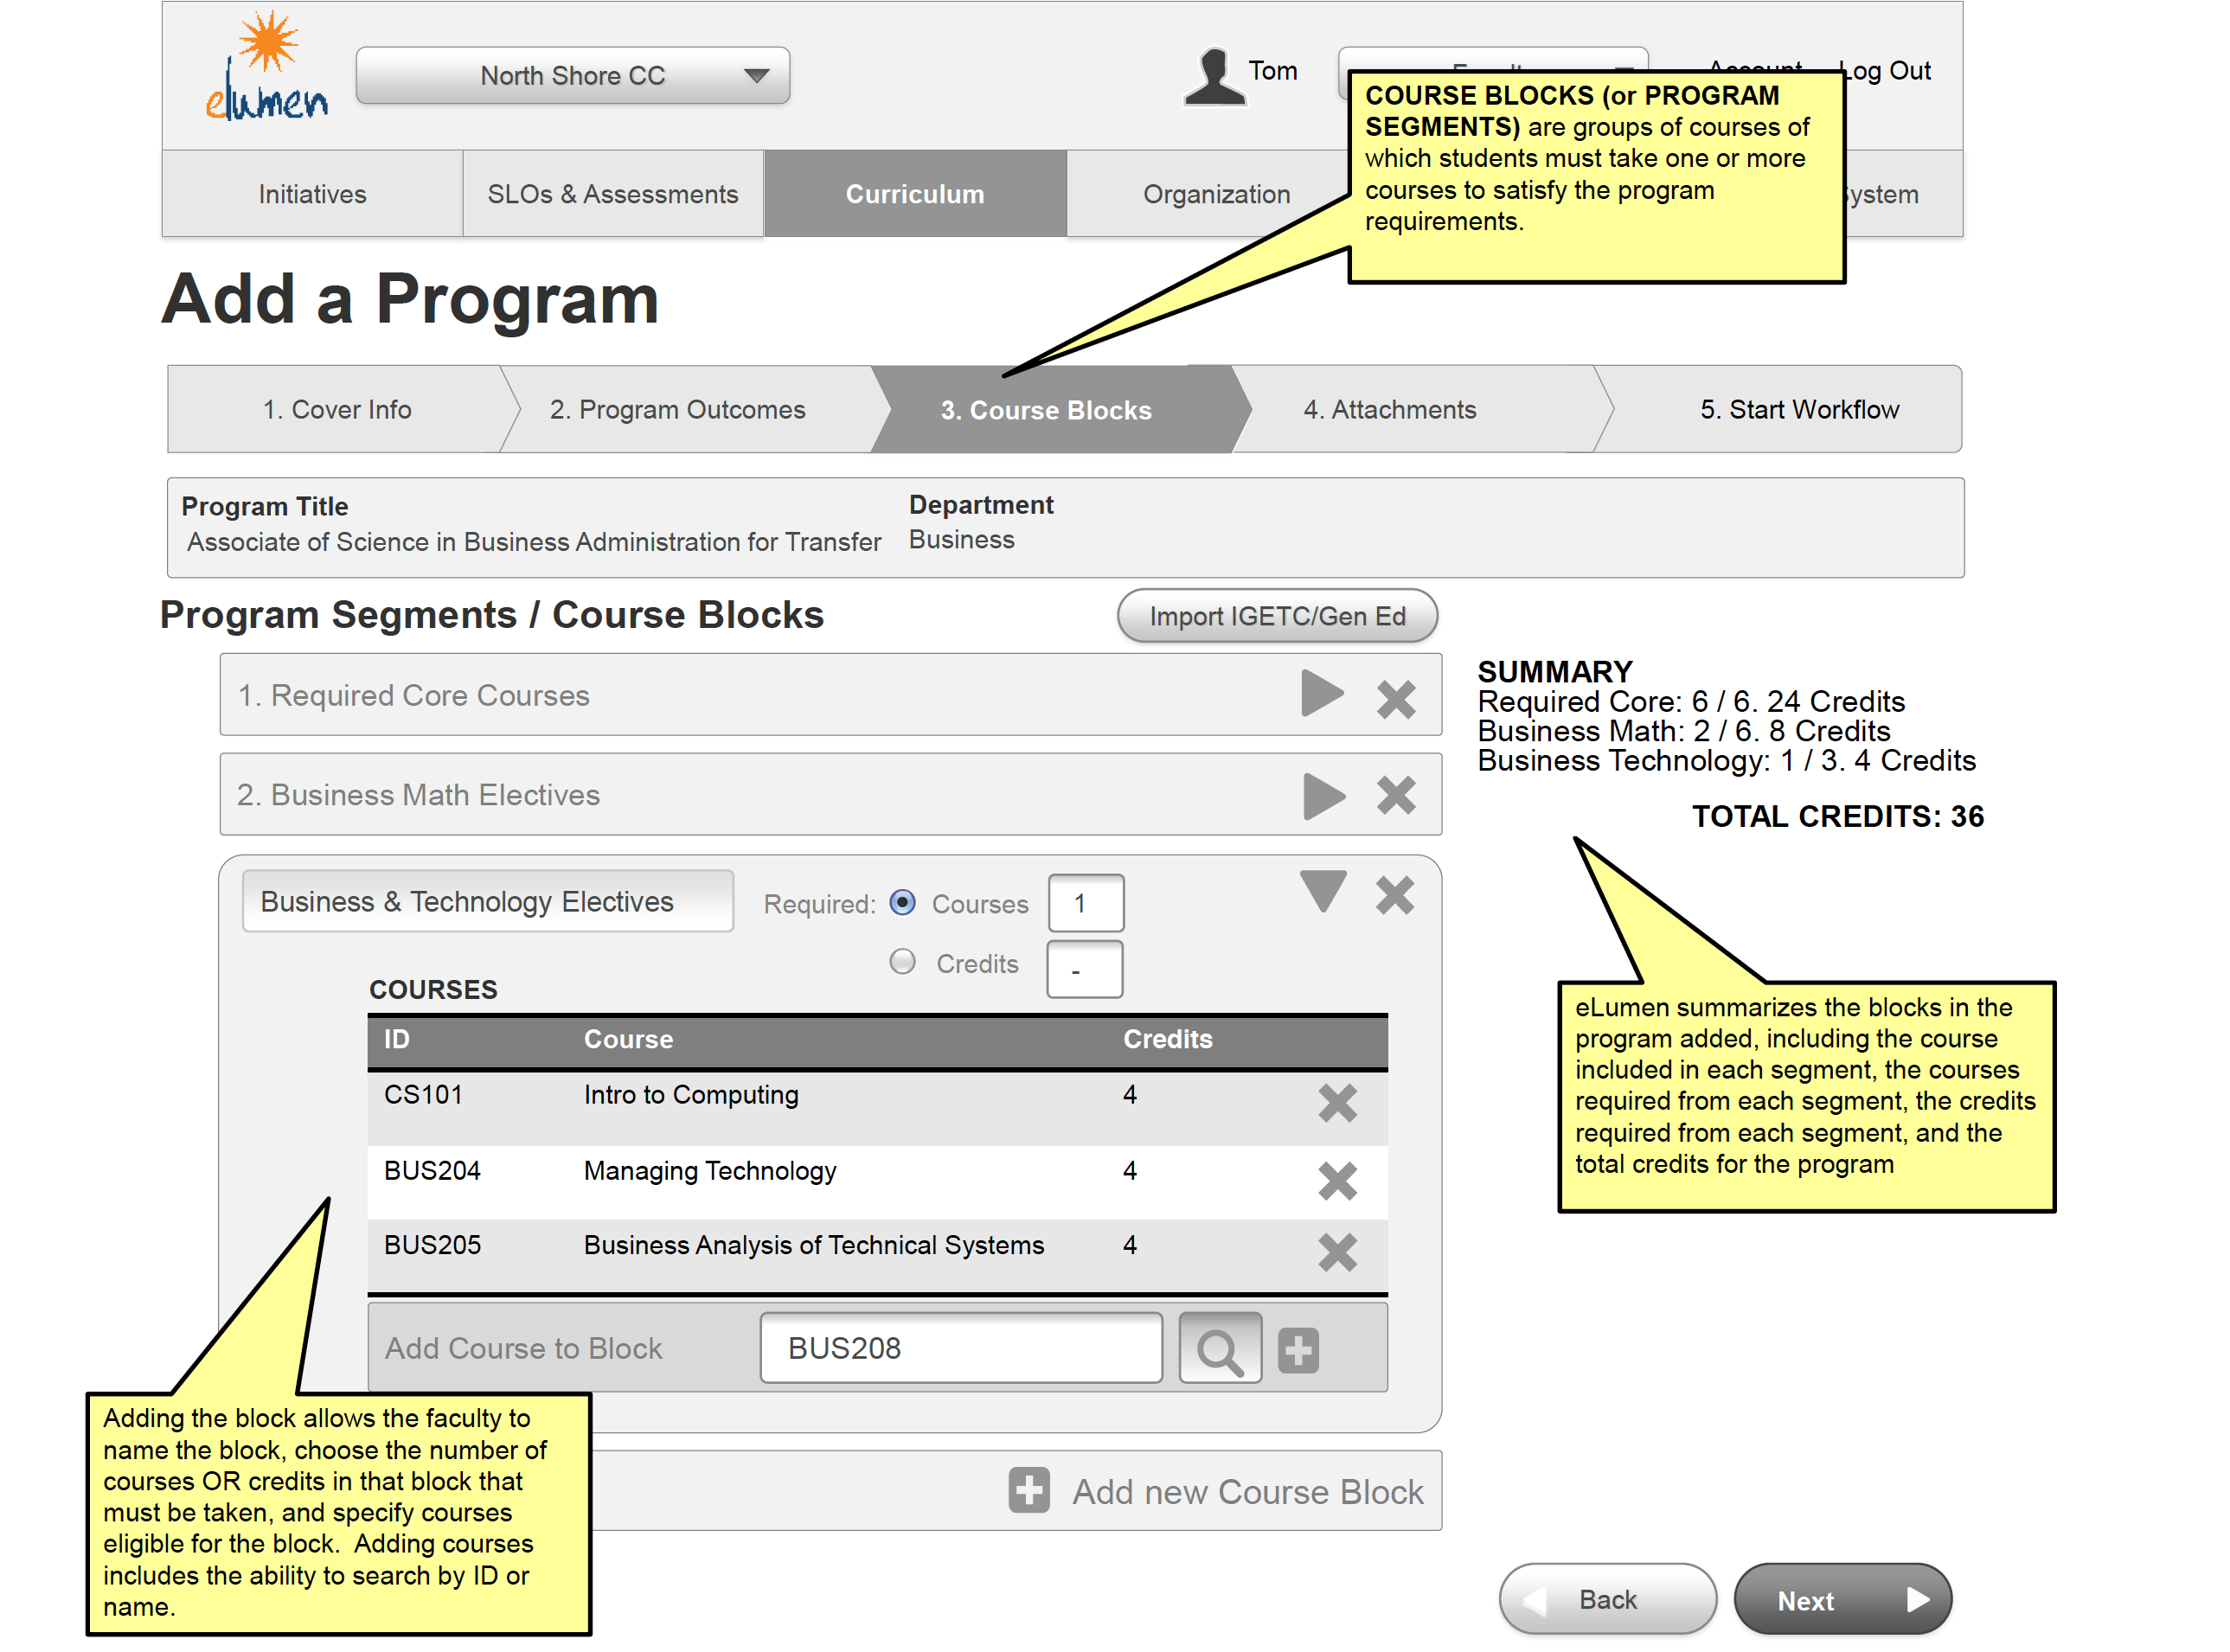
\includegraphics[width=125mm,scale=1]{Capitulos/DesarrollodelaAplicacion/Imagenes/program_course_blocks}
\caption{Mockup de la pantalla de bloques de cursos de programa.}
  \label{program_course_blocks}
\end{figure}

\subsection{Visualizar cambios en los campos}
La historia de usuario tiene como descripción lo siguiente \enquote{\textit{Como coordinador de departamento, me gustaría ser capaz de diseñar bloques de cursos para mis programas, para que de esta manera pueda diseñar la malla para mis programas de estudio}}. Y los criterios de aceptación consistían en el desarrollo de la pantalla que se puede apreciar en la figura \ref{visualize_changes}.

Como criterios de aceptación se encuentran los siguientes:
\begin{itemize}
	\item Los campos borrados se deben marcar en rojo.
	\item Los nuevos campos se deben marcar en verde.
	\item Se debe visualizar el estado anterior y el nuevo con una forma de identificar con el usuario que hizo la modificación.
	\item Limitado para los cambios del programa.
	\item Diseño de interfaz aprobada por el equipo de validación.
	\item Las diferencias limitadas a dos versiones.
\end{itemize}

Algunas de las tareas identificadas en la planificación de las iteraciones eran los siguientes:
\begin{itemize}
	\item Diseño e implementación del modelo de datos.
	\item Diseño e implementación de clases Java.
	\item Desarrollar la página de paso para creación de bloques de cursos en los diferentes flujos de trabajo.
	\item Desarrollar servicios de guardado y aprobación de la funcionalidad.
	\item Actualizar la plantilla de flujos de trabajo.
\end{itemize}

La historia fue finalizada en una iteración con una cantidad de 60 horas cargadas en el sistema.

\begin{figure}[H]
\centering
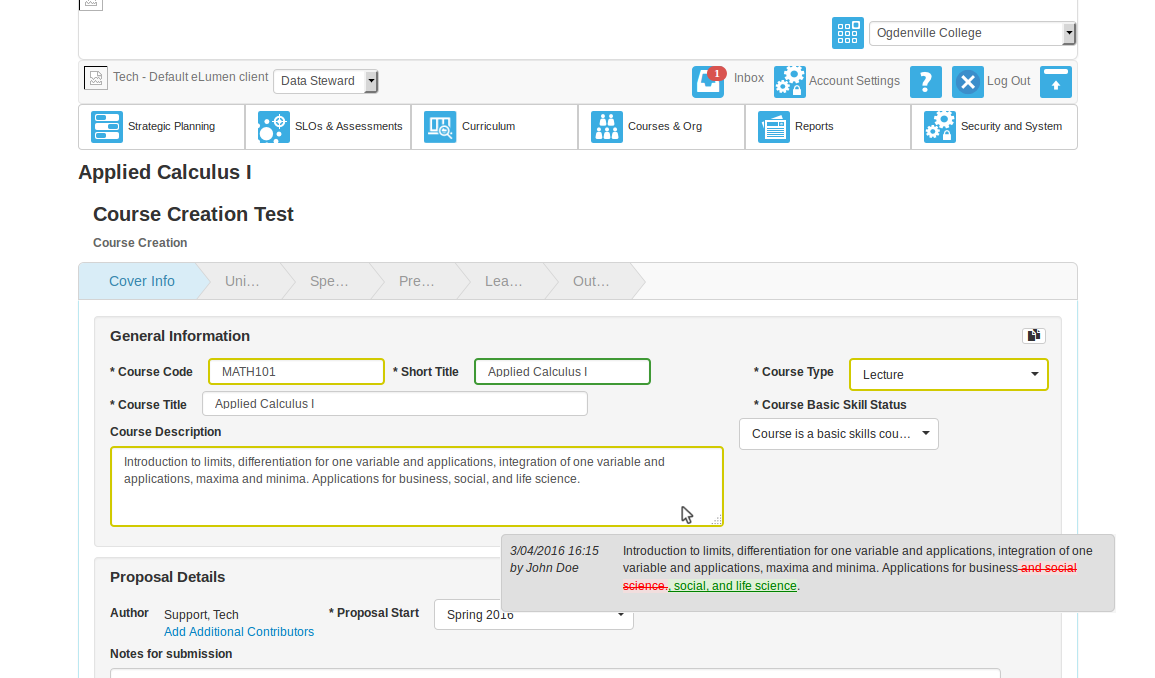
\includegraphics[width=125mm,scale=1]{Capitulos/DesarrollodelaAplicacion/Imagenes/visualize_changes}
\caption{Mockup de la pantalla de la funcionalidad de visualización de cambios.}
  \label{visualize_changes}
\end{figure}
